\begin{table}[H]
  \caption{Calibración por deciles de probabilidad predicha (conjunto de prueba).}
  \label{tab:calib}
  \tablabase\footnotesize
  \begin{tabular}{|l|c|c|}
    \hline
    \enc{Decil} & \enc{Probabilidad media} & \enc{Proporción observada} \\ \hline
    1 & 0.264 & 0.105 \\ \hline
    2 & 0.326 & 0.103 \\ \hline
    3 & 0.358 & 0.165 \\ \hline
    4 & 0.384 & 0.203 \\ \hline
    5 & 0.410 & 0.206 \\ \hline
    6 & 0.435 & 0.208 \\ \hline
    7 & 0.462 & 0.268 \\ \hline
    8 & 0.493 & 0.346 \\ \hline
    9 & 0.532 & 0.357 \\ \hline
    10 & 0.608 & 0.505 \\ \hline
  \end{tabular}
\end{table}

El error cuadrático de Brier es 0.205 (referencia con la prevalencia como única predicción: 0.186). \begin{figure}[H]
  \centering
  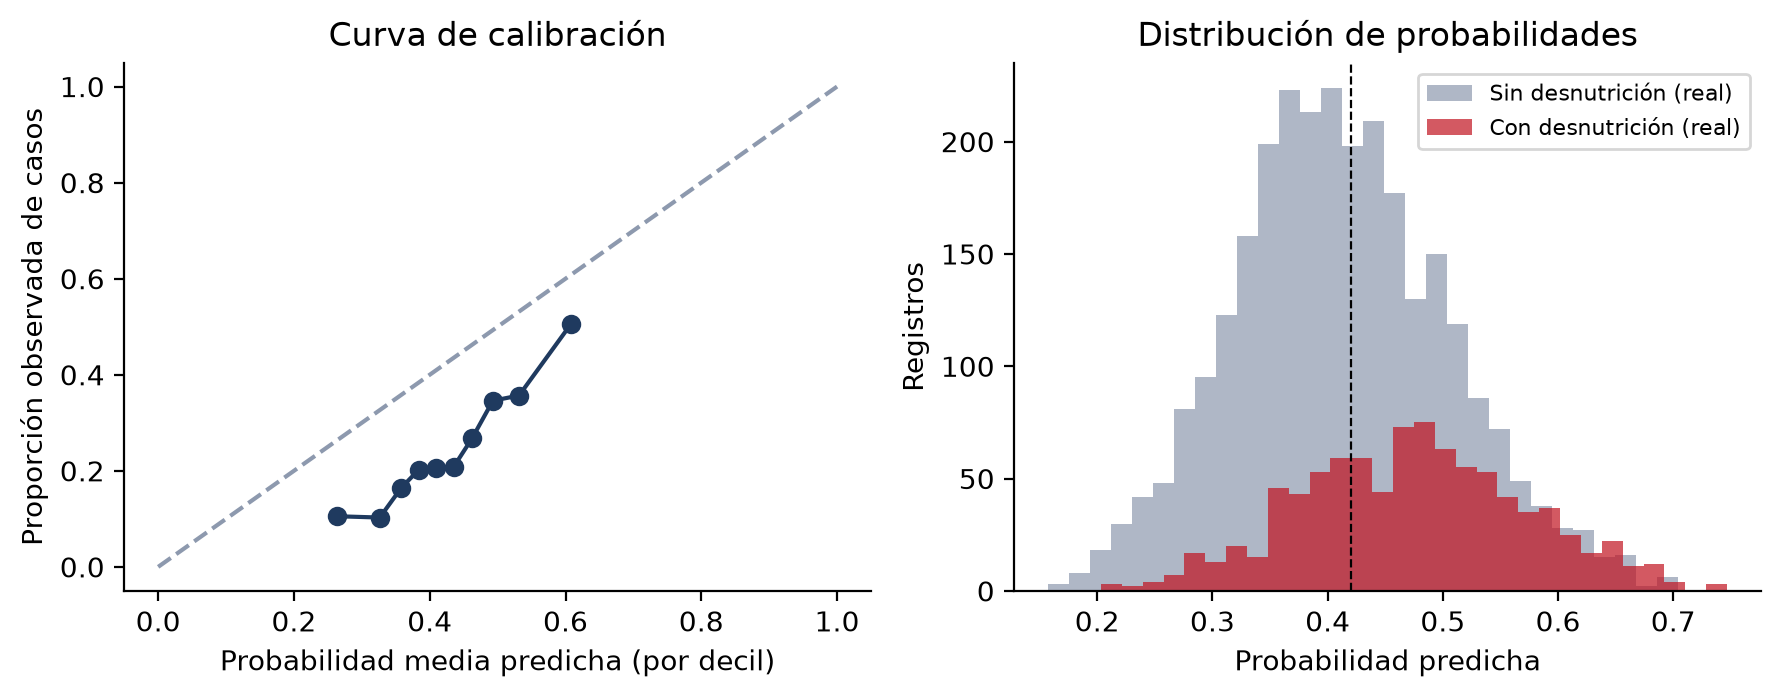
\includegraphics[width=0.95\textwidth]{figuras/anexo-calibracion.png}
  \caption{Curva de calibración y distribución de probabilidades predichas. Elaboración propia.}
  \label{fig:calibracion}
\end{figure}
